\chapter{Introdução}

\section{O que é Inteligência Artificial? E o que é a aplicação da ética em Inteligência Artificial?}

	
\begin{figure}
            \begin{center}
                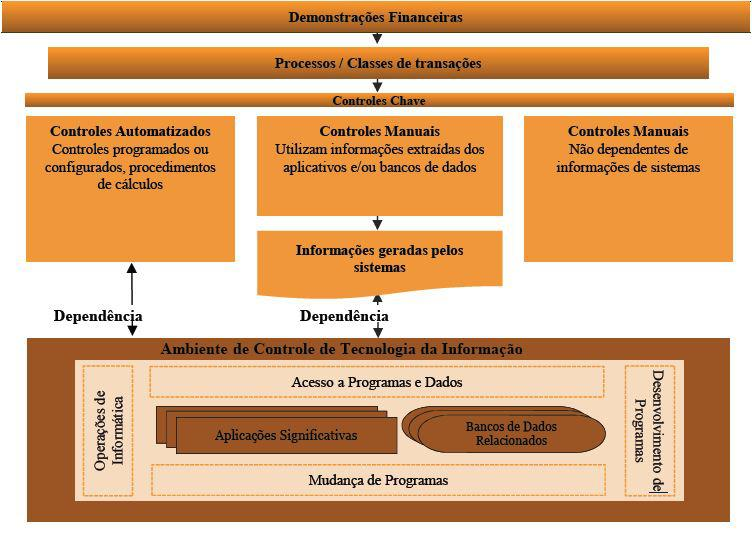
\includegraphics[width=0.7\textwidth]{Img1}
            \end{center}
            \caption{Como o ambiente de TI suporta as operações financeiras de um negócio hoje em dia.}
            \label{fig:Img1}
\end{figure}

\section{Inteligência Artificial}

    Lorem Ipsum Dolor Sit Amet\cite{SOX}
	
\subsection{Ética}

	Blablabla

\begin{itemize}
\item    Financeira (segundo a visão dos acionistas);
\item	 Cliente;
\item	 Processos internos de negócios;
\item	 Inovações.
\end{itemize}

Ao nos mostrar através de tais visões o que é mais crítico, esta framework permite direcionar recursos para os processos que adicionarão valor à empresa, de fato. A tecnologia entra nesta metodologia como uma valiosa peça para colocar o BSC em funcionamento, porém não como peça suficiente pelo fato desta ferramenta administrativa interagir com a cultura da corporação. Devido à sua grande complexidade e por envolver a estrutura empresarial como um todo, a adoção deste modelo deve partir da alta direção ou, a depender do caso, do presidente da empresa para que sua implementação seja viável.

Por ser um modelo razoavelmente flexível, permite ajustes temporários para se adequar ao objetivo final, que é a valorização da empresa. Esta visão ainda nos permite:

\begin{itemize}
\item Perspectivas diferentes da visão dos negócios;
\item Uma melhor monitoração e elaboração das estratégias;
\item Análise das relações de causa e efeito a partir de um macro indicador;
\item Alinhamento e compartilhamento da visão e metas desde o nível estratégico, passando pelo tático até alcançar o nível operacional;
\item Uma definição mais efetiva dos planos de ações;
\item Maior acurácia dos planos de ações a serem tomadas;
\item Maior eficiência do tempo a ser usado no processo de decisão
\item Colaboratividade através de mecanismos de compartilhamento de informações analíticas
\end{itemize}

Com a metodologia BSC como opção de gestão na Governança em TI, podemos realizar uma melhor avaliação e obter uma melhor gestão da organização não apenas de forma limitada apenas às medidas tradicionais de resultados e desempenho financeiros, mas também complementá-la com medidas de outras dimensões como a atenção na satisfação dos clientes, satisfação nos controles internos e capacidade de inovação e aprendizado. Tais dimensões adicionais nos garantem, se integradas, melhores resultados futuros e não apenas uma visão meramente dos resultados passados, obtidos apenas em uma perspectiva de gestão puramente financeira, mas também valorizando o capital que executa este serviço, seja ele humano ou seja ele automatizado.

\subsection{COBIT}

Criado em 1996 nos Estados Unidos, a metodologia COBIT (Control Objectives For Information and related Technology) foi criada pelo Information System Audit and Control Association (ISACA) com a intenção de ser um guia de boas práticas apresentado como um framework a partir de ferramentas de auditoria, funcionando como um um norte para a gestão da TI nas empresas, literalmente.

Esta metodologia apresenta padrões independentes, podendo ser implementada por qualquer tipo de negócio, com qualquer tipo de valor e de participação da tecnologia da informação dentro de sua cadeia produtiva. No momento, a versão utilizada do COBIT é a versão 5. Sua integração com outras frameworks foi ampliada com a intenção de aumentar a agregação entre estas ferramentas e, assim, possibilitar uma melhor produtividade. As frameworks que trabalham em conjunto com tal framework são em sua maior parte o ITIL, ISO, PMBOK (Projetct Management Body of Knowledge) e o TOGAF (The Open Group Architecture Framework).\cite{COBIT-4.1} \cite{SOX-COBIT}
	


        \begin{figure}
            \begin{center}
                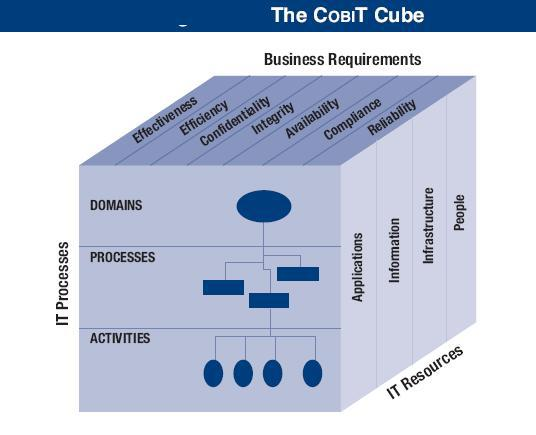
\includegraphics[width=0.7\textwidth]{Img2}
            \end{center}
            \caption{Cubo de aplicação do COBIT, mostrando seus processos, recursos e requisitos de negócios e sua abrangência. (COBIT 5, apud https://jane15cl.wordpress.com/2011/01/)}
            \label{fig:Img2}
        \end{figure}



Com o exame e aplicação do COBIT conforme as necessidades do negócio, este framework começou a ser extensivamente utilizado pelos auditores e gerentes por ser uma ferramenta que apresenta uma grande abrangência dos controles, porém de forma reduzida para que se possa visar uma melhor abrangência do ambiente a ser verificado.

Esta metodologia é voltada para três níveis distintos:
\begin{itemize}
    \item Gerentes que necessitam avaliar os riscos e controlar os investimentos de TI;
    \item Usuários que necessitam assegurar a qualidade dos serviços prestados para seus clientes, sejam estes internos ou externos;
    \item Auditores que precisam avaliar o trabalho da gestão de TI e aconselhar o controle interno da organização.
\end{itemize}

O principal foco é apontar onde possíveis melhorias devem ser realizadas e, nos casos em que seja necessário o exame, se possibilite o desenvolvimento e a implementação de novos procedimentos e controles.  Desta forma, uma política de revisão constante com o objetivo de manter a eficácia dos mesmos é essencial.

Podemos aqui apresentar algumas recomendações sobre os controles:
\begin{itemize}
    \item Os controles devem ser os mais simples e objetivos possíveis;
    \item As atualizações de revisões devem ser devidamente documentadas e armazenadas;
    \item O processo de revisão deve perturbar o mínimo possível as funções de rotina, ou seja, a revisão de tal processo não deve gerar um grande impacto no negócio de forma a diminuir sua eficiência;
    \item O processo de revisão deve ser automatizado e suas atualizações produzidas sistematicamente, de preferência;
    \item A frequência da revisão dos itens de controle se dá de acordo com a conformidade e a necessidade do negócio, podendo ser semanal, mensal, trimestral, etc.
\end{itemize}
\subsection{ITIL}	
	\cite{ITIL-OVERVIEW}

	Criado no final dos anos 1980 pela Central Computing and Telecommunications Agency, hoje Office for Government Commerce para o governo britânico, o ITIL (Information Technology Infrastructure Library) reúne um conjunto de recomendações, sendo dividido em dois blocos que por sua vez se subdividem-se em cinco outros blocos:
 
Entrega de serviço, que engloba os tópicos de gerenciamento de níveis de serviço, gerenciamento de capacidade, gerenciamento de finanças, gerenciamento de disponibilidade e continuidade de serviço e;


Suporte de serviços, que engloba o service desk, o gerenciamento de incidentes, o gerenciamento de problemas, o gerenciamento de configurações, o gerenciamento de mudanças e o gerenciamento de versões.

	Por sua grande flexibilidade, a adoção do ITIL traz grandes benefícios, uma vez que ele não define quais processos devem ser implementados, mas sim mostra quais são as melhores práticas a ser utilizadas. De forma clara, podemos mostrar alguns resultados decorrentes de sua implementação, tais como:

Definição dos ciclos de vida dos processos;
Análise e classificação dos erros;
Aumento no grau de segurança do usuário;
Organização de métodos de trabalho;
Geração de contínuas melhorias e referências para novos usuários;
Contribuição como facilitador e integrador entre as áreas de trabalho;
Disponibilização dos recursos tecnológicos em tempo integral;
Restauração da operação normal do serviço;
Avaliação de impactos de mudança;
Obtenção e uso de indicadores;
Entre outros.

	Complementar ao COBIT, o ITIL é uma série de documentos usada como auxílio à implementação de uma estrutura de gerenciamento de serviços de TI, uma biblioteca que descreve detalhadamente as melhores práticas de gestão, elaboradas especificamente para a área de TI. Os pontos focados apresentam as melhores práticas para a central de atendimento, para o gerenciamento de incidentes, para o gerenciamento de problemas e também para o gerenciamento financeiro para serviços de TI, com a finalidade de ajudar no objetivo de definição do gerenciamento de serviços e suas aplicações para empresas especificas, independente do aplicativo ou plataforma e, sendo assim, aplicável a qualquer empresa.

\subsection{CMMI}

	CMMI é um modelo de referência que possui práticas necessárias à maturidade em disciplinas específicas, podendo estas ser genéricas ou específicas. Ele se destina a auxiliar empresas a melhorar a produtividade dos processos de desenvolvimento de software e a organizar o funcionamento dos ambientes de tecnologia de informação. Esta metodologia ajuda a mostrar quais metas devem ser alcançadas através da quantificação, orientação e qualificação dos estágios de maturidade da empresa.
	O CMMI é definido em quatro níveis de maturidade para os ambientes de desenvolvimento de software (incompleto, inicial, repetível e definido), sendo cada um destes composto por um conjunto de áreas-chave de processos que descrevem as questões e os grandes temas que devem ser abordados e resolvidos para o alcance de um determinado nível de maturidade definido segundo o framework. 
	\cite{CMMI}
	
\section{Processos utilizados na auditoria de sistemas}
	
	Quando a Tecnologia da Informação é usada para iniciar, gravar, processar e reportar transações ou outros dados financeiros para a sua inclusão nos relatórios financeiros, devemos considerar como tais informações (e seu gerenciamento, caso sejam relevantes), estão mapeadas, bem como se estão de acordo com os processos de negócios (incluindo o processo da demonstração financeira em si), com os sistemas e ambientes computacionais para cada unidade de gerenciamento significante, seu entendimento e avaliação. Desta forma, verifica-se:
\begin{itemize}
    \item As principais características dos sistemas e ambientes;
    \item Gerenciamento dos sistemas de informações e tecnologia;
    \item Mudanças de sistemas e ambientes significantes que podem impactar na geração do relatório financeiro;
    \item Problemas reconhecidos dos sistemas;
    \item Como a instituição tem respondido aos riscos de distorções materiais que podem surgir dos sistemas de informação e tecnologia.
\end{itemize}


	Ao se analisar tais aspectos, se fazem necessárias a avaliação dos controles da área da tecnologia, da eficiência dos sistemas de informação, e a verificação e cumprimento das legislações e normativos aos quais estão sujeitos e da gestão eficaz dos recursos de informática. Para a análise destes processos, quatro atividades são realizadas, quais sejam: a verificação de acessos a programas e dados, o desenvolvimento dos programas utilizados pela empresa, a gerência de mudanças e as operações de informática, as quais descreveremos logo a seguir.	

\subsection{Acesso a Programas e Dados}

	Este elemento agrupa controles relacionados ao gerenciamento de acesso a sistema e dados, tanto lógicos quanto físicos. O foco destes controles é a redução de risco de acesso inapropriado ou não autorizado a sistemas de informações e a prevenção da execução ou ocultação de erros ou irregularidades. As áreas de controle relevantes a este elemento incluem:
\begin{itemize}
\item    \subsubsection{Políticas de TI}
	Uma política de segurança formalizada tem sido adotada, a qual é revisada e aprovada pela gerência. A política deve ser comunicada a todos na organização.
\item	\subsubsection{Data Center}
	O acesso físico ao Data Center é restrito ao pessoal apropriado.
\item	\subsubsection{Parâmetros de senhas}
	Os parâmetros de senhas da rede estão apropriadamente configurados, assim como para os sistemas críticos e sua relevante infraestrutura (como banco de dados e sistemas operacionais).
\item	\subsubsection{Contas superusuários (root)}
	Acessos a contas root ou privilegiadas da rede, sistemas críticos, sistemas operacionais e banco de dados são restritos a um determinado grupo de adminstradores de sistemas.
\item	\subsubsection{Provisão ou modificação de acesso ao usuário}
	Existem procedimentos predefinidos para outorgar ou modificar acessos e direitos de acesso para usuários em sistemas relevantes ao negócio. Tais procedimentos exigem uma aprovação formal para a garantia ou modificação destes.
\item	\subsubsection{Retirada de acesso}
	Existem procedimentos para a restrição do acesso e seus direitos aos usuários para os sistemas relevantes. A revogação destes acessos é realizada de forma eficiente e em tempo hábil.
\item	\subsubsection{Revisões periódicas de acesso a usuários}
	Revisões periódicas são executadas de forma a identificar se os usuários ativos estão com seus devidos acessos e, caso não estejam, adequá-los de acordo com as políticas internas da empresa, limitando o acesso à rede, aos sistemas e à infraestrutura.
\end{itemize}
\subsection{Desenvolvimento de Programas}
	Este elemento é relevante para os controles de desenvolvimento de novas aplicações ou sistemas. O objetivo destes controles é garantir que novos sistemas que são desenvolvidos ou adquiridos sejam autorizados, testados, aprovados, devidamente implementados e documentados.
	
\begin{itemize}
\item	\subsubsection{Metodologias}
	O ciclo de vida do desenvolvimento de sistemas segue uma metodologia para a aquisição ou desenvolvimento de novos sistemas ou aplicações. De maneira similar ao gerenciamento de mudança de programas, todas as novas aquisições ou desenvolvimentos são aprovados, testados e documentados.
\end{itemize}

\subsection{Mudança de Programas}

	Este elemento é relevante para os controles de mudança de aplicações ou de sistemas. O objetivo destes controles é garantir que novas versões desenvolvidas ou adquiridas sejam autorizadas, testadas, aprovadas, devidamente implementadas e documentadas.
\begin{itemize}
\item	\subsubsection{Gerenciamento de mudança de programas}
	As mudanças realizadas nos sistemas seguem políticas de gerenciamento de mudanças e procedimentos estabelecidas pela gerência (inclusive mudanças de configurações ou mudanças emergenciais). Estas mudanças são registradas, aprovadas e testadas antes de serem promovidas para o ambiente de produção.
	
\item	\subsubsection{Segregação de cargos}
	Deve ser garantida uma segregação de cargos entre os desenvolvedores, os homologadores e o ambiente de produção, sendo tolerável que o desenvolvedor ou o usuário final possa ser também um homologador.
\end{itemize}
\subsection{Operações de Informática}

	Este elemento agrupa os controles ligados a assuntos operacionais, como backups e procedimentos em batch (procedimentos em lote).  O objetivo destes controles é garantir que o processamento do sistema ou aplicação esteja apropriadamente autorizado e agendado, e que as variações de agendamento sejam identificadas e resolvidas. As áreas de controles relevantes a este elemento incluem:
    
\begin{itemize}
\item	\subsubsection{ Processamento/Monitoramento de trabalhos em batch}

	Os procedimentos de monitoramento são desenvolvidos para prover garantias razoáveis em relação à completude e à oportunidade do processamento de dados no sistema.

\item	\subsubsection{Gerenciamento de incidentes}

	A organização tem processos para gerenciamento de incidentes para tratar incidentes de prioridade média ou alta dentro de um prazo preestabelecido.
	
\item	\subsubsection{Backup de sistemas}
	
	As rotinas de backup e recuperação são implementadas pela gerência de modo a garantir que os dados, transações e programas necessários para a geração dos relatórios financeiros possam ser devidamente recuperados. Os procedimentos de backup e restore são testados periodicamente.
	
\item	\subsubsection{Armazenamento remoto}
	
	Procedimentos devem ser estabelecidos para armazenar o backup em um estabelecimento remoto (podendo este ser de terceiros ou não) de maneira periódica. O acesso a estes locais é gerenciado de forma restrita para pessoas autorizadas segundo as responsabilidades profissionais.
\end{itemize}

O processo de auditoria visa garantir a qualidade dos sistemas e serviços e consequentemente a confiabilidade das instituições auditadas. O alto custo deste processo requer atenção à otimização do mesmo. A correta aplicação da engenharia de software permite não só maior confiabilidade dos sistemas gerados, facilitando o processo de auditoria, como também procura atestar uma melhor compreensão do sistema auditado, seja pela presença de documentação relevante, seja pela correta estruturação daquele. Estas qualidades permitem também maior facilidade de atualização ou alteração do sistema, tornando mais eficiente a adequação do mesmo a padrões de qualidade ainda não respeitados e à correção de erros identificados ao longo do processo de auditoria.
	
Mas como esta breve introdução pode ter a ver com a educação nas instituições? Será que podemos nos permitir questionar que tais métodos podem não somente ajudar a instituição a ter ganhos em eficiência, mas não somente no quesito sistêmico? Ora, muitas vezes vemos várias empresas e instituições (afinal a governança não deve servir apenas para o mercado financeiro, na visão de lucros) implantarem políticas organizacionais, e até mesmo políticas focadas para que a TI seja, de fato, o suporte do negócio. 

Mas como tem sido a aplicação destas políticas para os funcionários? Eles tem aceito isto de forma unilateral, únicamente pela necessidade de se manter no trabalho? A empresa tem visto tal problema também da ótica do "chão de fábrica"? Pois sempre é válido pensarmos que se temos ferramentas que podem servir para aumentar nossos ganhos, usá-la a nosso favor. Porém será que elas são suficientes por si só, sem nenhum processo de ensino e aprendizagem para não somente começar o trabalho, mas principalmente mantê-lo e ajudar a empresa a atacar problemas que podem ser não somente de cunho estrutural da mudança em si, mas também da mentalidade das pessoas que adentram ao negócio?

Este serão alguns dos questionamentos que vamos tentar esclarecer ao longo do nosso trabalho. Porém antes, para tanto iremos passar por alguns tópicos para nos ajudar a melhor estruturar nosso trabalho. Teremos que primeiro conhecer um pouco mais a fundo o que é a governança em TI, quais são os processos que supostamente precisam acompanhar para a correta implantação do sistema e das novas políticas, quais ferramentas educacionais poderão nos ajudar durante estes processos e se eles são suficientes. Vamos acompanhar também um estudo de caso de gestão de mudança e como uma ferramenta educacional ajudou durante este processo. 

Veremos também ao longo deste trabalho, como estes casos são mais comuns na literatura do que imaginamos (tanto quanto da nossa parte não termos tido facilidades em achar trabalhos produzidos no país sobre esta área) e quais foram as soluções encontradas. Esperamos ao final deste trabalho esclarecer como a educação tem a ver com a governança em TI, e como a informática pode fornecer um valioso suporte para tais políticas que iremos estudar.